\begin{pastexam}[label={px:ccu-115-swa-14}]{中正資工所甲組 115 學年度 第 24 題}
（複選；全對才給分）

(3\%) (\qquad) Determine the order in which vertices are selected by Dijkstra's algorithm on the
graph below, starting from source vertex $A$. If two unvisited vertices have the same tentative
distance, select the vertex with the smaller alphabetical label first.
\begin{center}
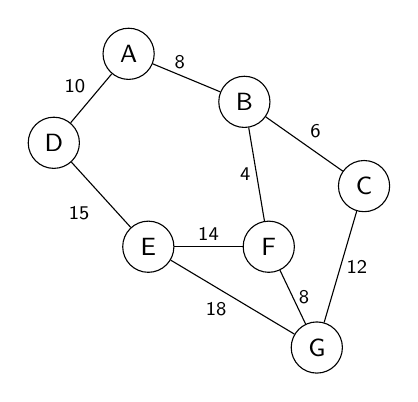
\begin{tikzpicture}[x=1cm,y=1cm,v/.style={circle,draw,minimum size=6.5mm,inner sep=1pt,font=\small\sffamily},lab/.style={font=\scriptsize\sffamily,inner sep=2pt}]
\node[v] (A) at (1.64,-0.58) {A};
\node[v] (B) at (3.11,-1.19) {B};
\node[v] (D) at (0.69,-1.71) {D};
\node[v] (C) at (4.63,-2.26) {C};
\node[v] (E) at (1.89,-3.03) {E};
\node[v] (F) at (3.42,-3.03) {F};
\node[v] (G) at (4.03,-4.31) {G};
\draw (A) -- node[lab,above,pos=0.4]{8} (B);
\draw (A) -- node[lab,above left]{10} (D);
\draw (B) -- node[lab,above right]{6} (C);
\draw (B) -- node[lab,left]{4} (F);
\draw (D) -- node[lab,below left=2pt]{15} (E);
\draw (E) -- node[lab,above]{14} (F);
\draw (E) -- node[lab,below left]{18} (G);
\draw (F) -- node[lab,right]{8} (G);
\draw (C) -- node[lab,right]{12} (G);
\end{tikzpicture}
\end{center}
(a)~(A, D, B, E, F, C, G) \qquad (b)~(A, B, F, G, C, D, E) \qquad (c)~(A, D, B, F, G, C, E)\\
(d)~(A, B, D, F, C, G, E) \qquad (e)~none of the above
\end{pastexam}

\begin{pastsoln}
答案：只有 (d)。

圖是無向圖，每條邊兩個方向都能走。 從 A 執行 Dijkstra 演算法（資結書虛擬碼~25.3），平手時取
字母小的（題目的規則）。 每一列是取出那個頂點、鬆弛完它的鄰居之後的 $d$；粗體是這一輪取出的
頂點，$*$ 表示已經取出過：
\begin{center}
\small
\begin{tabular}{cc*{7}{c}}
\toprule
輪 & 取出 & A & B & C & D & E & F & G \\
\midrule
1 & A & \textbf{0} & 8 & $\infty$ & 10 & $\infty$ & $\infty$ & $\infty$ \\
2 & B & $*$ & \textbf{8} & 14 & 10 & $\infty$ & 12 & $\infty$ \\
3 & D & $*$ & $*$ & 14 & \textbf{10} & 25 & 12 & $\infty$ \\
4 & F & $*$ & $*$ & 14 & $*$ & 25 & \textbf{12} & 20 \\
5 & C & $*$ & $*$ & \textbf{14} & $*$ & 25 & $*$ & 20 \\
6 & G & $*$ & $*$ & $*$ & $*$ & 25 & $*$ & \textbf{20} \\
7 & E & $*$ & $*$ & $*$ & $*$ & \textbf{25} & $*$ & $*$ \\
\bottomrule
\end{tabular}
\end{center}
幾個要看清楚的地方：第 2 輪 B 鬆弛 C 得 $8 + 6 = 14$、F 得 $8 + 4 = 12$；第 3 輪 D 鬆弛 E 得
$10 + 15 = 25$；第 4 輪 F 鬆弛 E 得到 $12 + 14 = 26$，不比 $25$ 小，不更新，鬆弛 G 得 $12 + 8 = 20$；
第 5 輪 C 鬆弛 G 得到 $14 + 12 = 26$，不比 $20$ 小；第 6 輪 G 鬆弛 E 得到 $20 + 18 = 38$，也不更新。
每一輪剩下的頂點裡最小的 $d$ 都只有一個，這張圖用不到平手規則。 取出的順序是
A, B, D, F, C, G, E。
\begin{itemize}
\item (a) 錯：第 2 個取出的應該是 $d = 8$ 的 B，不是 $d = 10$ 的 D。
\item (b) 錯：前兩個 A, B 對，但第 3 個應該是 D（$10$），不是 F（$12$）。
\item (c) 錯：第 2 個就錯了，理由同 (a)。
\item (d) 對：和上表相同。
\item (e) 錯：(d) 是對的。
\end{itemize}
\end{pastsoln}
